\documentclass[11pt,a4paper]{article}

\usepackage[margin=2.5cm]{geometry}
\usepackage{graphicx}
\usepackage{booktabs}
\usepackage{hyperref}
\usepackage{float}
\usepackage{caption}
\usepackage{subcaption}
\usepackage{xcolor}
\usepackage{enumitem}
\usepackage{listings}
\usepackage{amsmath}

\hypersetup{
    colorlinks=true,
    linkcolor=blue!70!black,
    citecolor=blue!70!black,
    urlcolor=blue!70!black
}

\lstset{
    basicstyle=\ttfamily\small,
    backgroundcolor=\color{gray!10},
    frame=single,
    framerule=0pt,
    breaklines=true,
    language=Python,
    keywordstyle=\color{blue!70!black}\bfseries,
    stringstyle=\color{red!70!black},
    commentstyle=\color{green!50!black}\itshape
}

\title{\vspace{2cm}\textbf{\LARGE Market Sentiment Classification\\of Financial Tweets}\vspace{1cm}}
\author{
    \textbf{Text Mining --- Spring Semester 2025/2026}\\[0.5cm]
    Group XX
}
\date{June 2026}

\begin{document}

\maketitle
\thispagestyle{empty}
\newpage
\setcounter{page}{1}
\tableofcontents
\newpage

%==============================================================================
\section{Data Exploration}
%==============================================================================

\subsection{Dataset Overview}

The dataset consists of \textbf{9,543 financial tweets} annotated with three sentiment classes. The training data exhibits significant class imbalance:

\begin{itemize}[noitemsep]
    \item \textbf{Neutral}: 6,174 tweets (64.7\%)
    \item \textbf{Bullish}: 1,928 tweets (20.2\%)
    \item \textbf{Bearish}: 1,441 tweets (15.1\%)
\end{itemize}

A held-out test set of \textbf{2,486 tweets} is used for final prediction. The average tweet length is approximately 86 characters, and the corpus contains rich financial vocabulary including stock tickers (e.g., \texttt{\$TSLA}, \texttt{\$AAPL}), company names, and market terminology.

\subsection{Class Distribution and Text Statistics}

The class imbalance (Neutral dominating at nearly 65\%) poses challenges for classification, particularly for the minority Bearish class. Tweet lengths follow a right-skewed distribution, with most tweets being concise market commentary.

\begin{figure}[H]
    \centering
    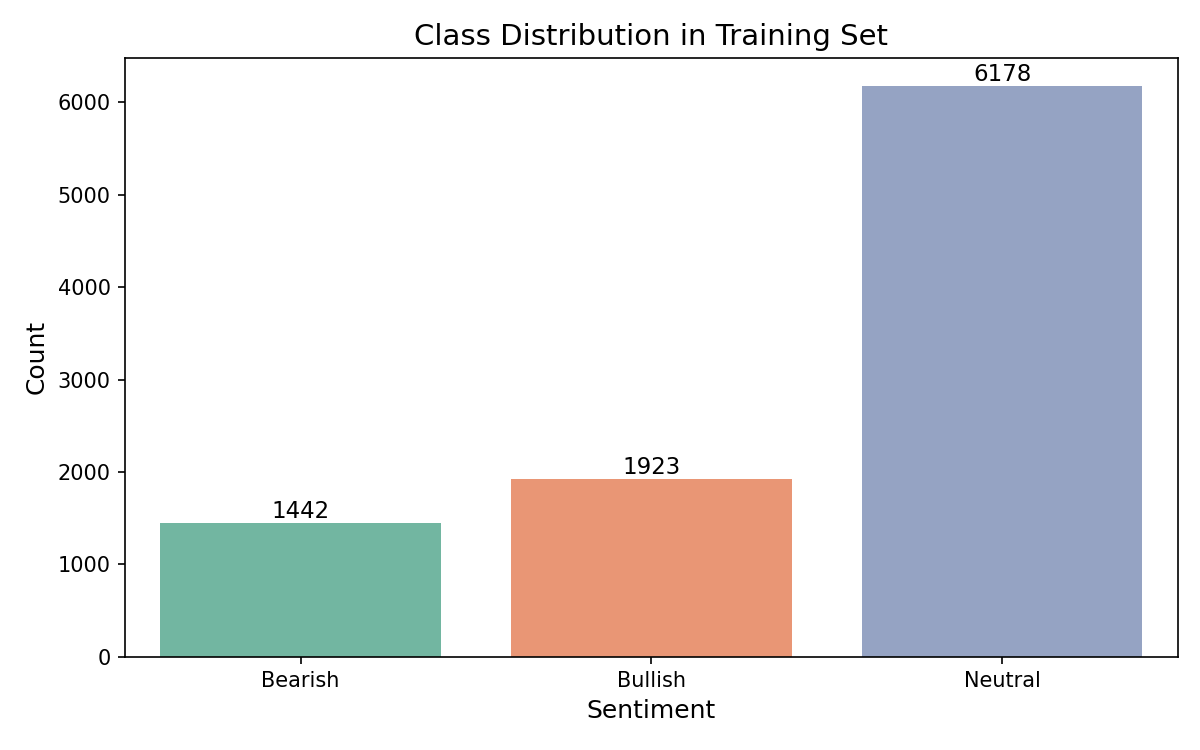
\includegraphics[width=0.7\textwidth]{../src/outputs/figures/class_distribution.png}
    \caption{Distribution of sentiment classes in the training dataset.}
    \label{fig:class_dist}
\end{figure}

\subsection{Topic Modeling with BERTopic}

We applied BERTopic~\cite{grootendorst2022bertopic} to discover latent themes in the corpus. The model identified \textbf{14 distinct topics}:

\begin{table}[H]
\centering
\small
\begin{tabular}{ll}
\toprule
\textbf{Topic} & \textbf{Topic} \\
\midrule
1. Stock earnings \& results & 8. Streaming wars (Netflix, Disney+) \\
2. Coronavirus \& trade war & 9. Energy \& oil markets \\
3. Federal Reserve \& employment & 10. Boeing \& aerospace \\
4. Brexit \& European markets & 11. 5G \& telecommunications \\
5. Retail sector performance & 12. Cryptocurrency mentions \\
6. Banking \& financial services & 13. IPO \& tech valuations \\
7. Tesla \& electric vehicles & 14. General market commentary \\
\bottomrule
\end{tabular}
\end{table}

Figure~\ref{fig:wordclouds} presents word clouds for each sentiment class, revealing distinctive vocabulary patterns.

\begin{figure}[H]
    \centering
    \begin{subfigure}[b]{0.32\textwidth}
        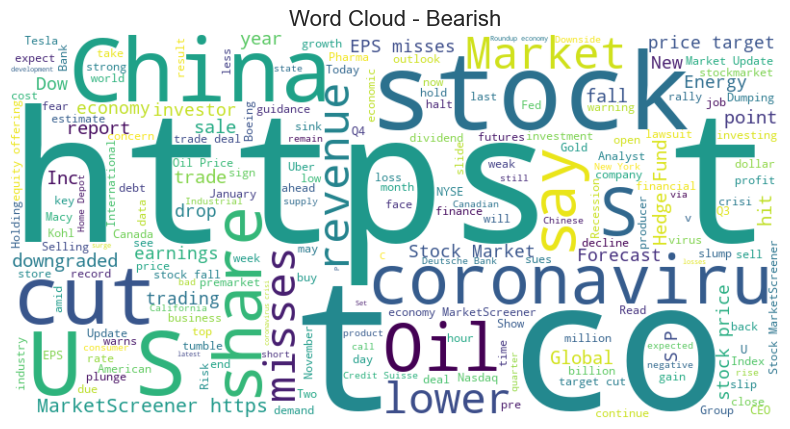
\includegraphics[width=\textwidth]{../src/outputs/figures/wordcloud_bearish.png}
        \caption{Bearish}
    \end{subfigure}
    \hfill
    \begin{subfigure}[b]{0.32\textwidth}
        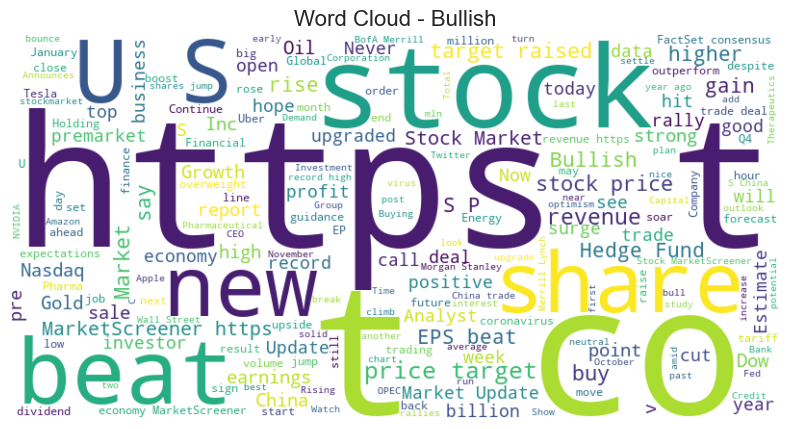
\includegraphics[width=\textwidth]{../src/outputs/figures/wordcloud_bullish.png}
        \caption{Bullish}
    \end{subfigure}
    \hfill
    \begin{subfigure}[b]{0.32\textwidth}
        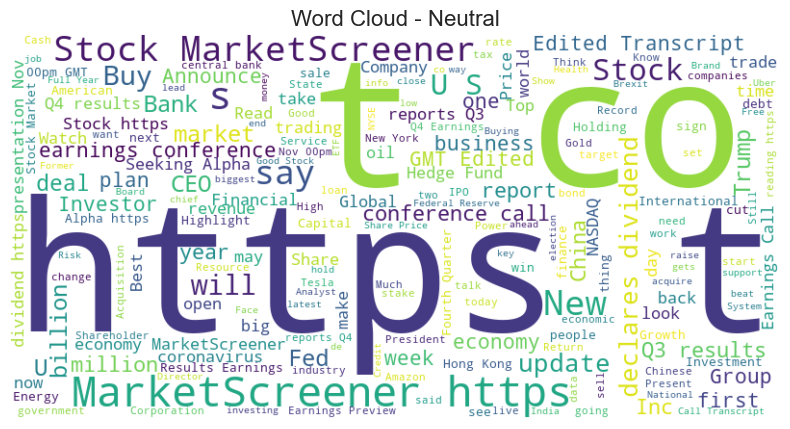
\includegraphics[width=\textwidth]{../src/outputs/figures/wordcloud_neutral.png}
        \caption{Neutral}
    \end{subfigure}
    \caption{Word clouds for each sentiment class revealing distinctive vocabulary patterns.}
    \label{fig:wordclouds}
\end{figure}

\begin{figure}[H]
    \centering
    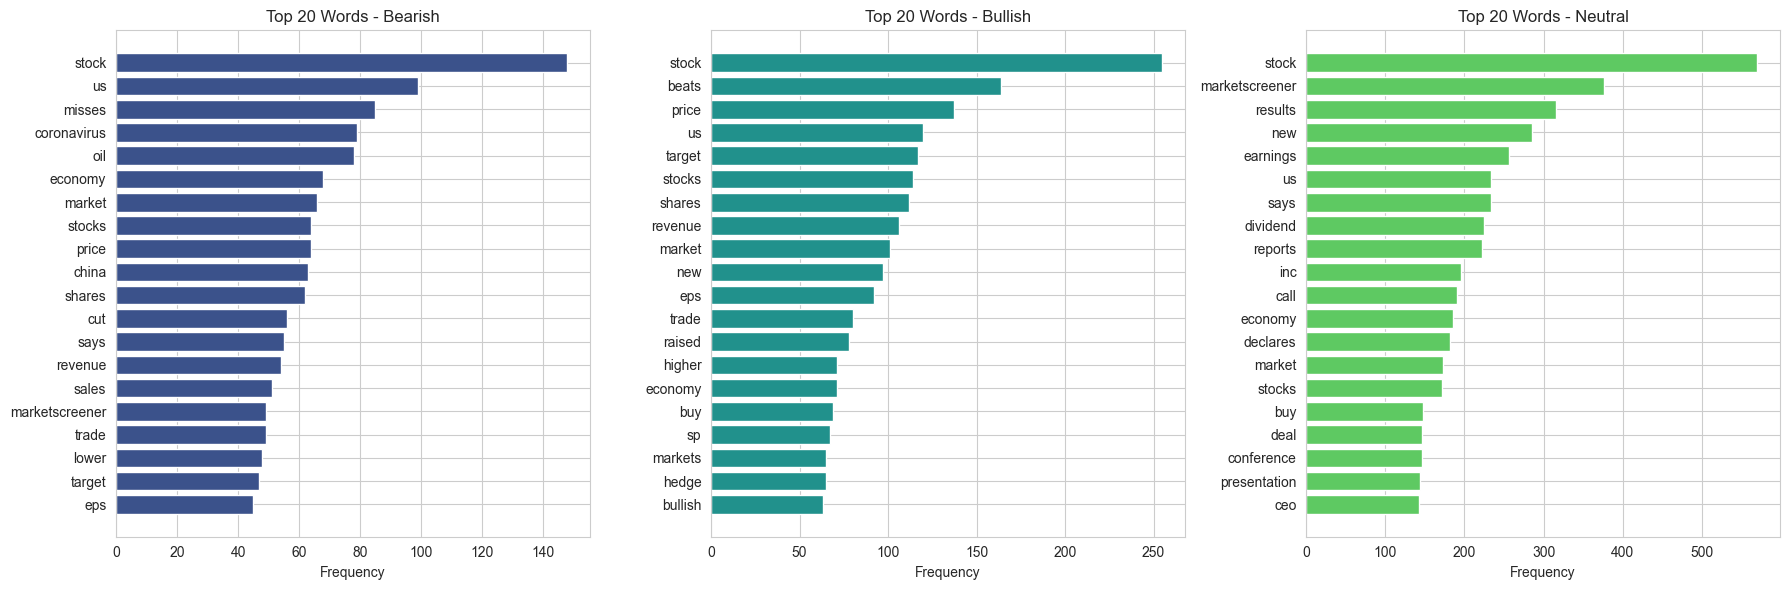
\includegraphics[width=0.9\textwidth]{../src/outputs/figures/top_words_per_class.png}
    \caption{Top 20 most frequent words per sentiment class after preprocessing.}
    \label{fig:top_words}
\end{figure}

%==============================================================================
\section{Corpus Split}
%==============================================================================

We performed a stratified 80/20 train/validation split using scikit-learn's \texttt{train\_test\_split} with \texttt{stratify=y}. Stratification ensures proportional class representation in both sets, which is critical given the 65\% Neutral class imbalance. The resulting split yields a \textbf{training set of 7,634 tweets} and a \textbf{validation set of 1,909 tweets}. The same split is used consistently across all experiments to ensure fair comparison between models.

%==============================================================================
\section{Data Preprocessing}
%==============================================================================

We implemented a multi-stage preprocessing pipeline with five techniques, designed to clean financial tweet text while preserving semantically meaningful content.

\subsection{Text Normalization (Entity Masking)}

Financial tweets contain a high density of named entities (tickers, companies, prices, URLs, user mentions) that create extreme vocabulary sparsity. For example, over 1,200 unique ticker symbols appear in the corpus, each occurring only a handful of times. Rather than removing these entities (which would lose structural information), we replace them with \textbf{semantic mask tokens} that preserve the entity's \textit{role} while abstracting away its specific identity. This allows the model to learn that the presence of a ticker is relevant to sentiment, regardless of whether it is \$TSLA or \$AAPL.

A custom \texttt{TextNormalizer} class implements the following regex-based replacements:

\begin{table}[H]
\centering
\caption{Entity masking rules applied during preprocessing.}
\label{tab:masking}
\begin{tabular}{lll}
\toprule
\textbf{Pattern} & \textbf{Mask Token} & \textbf{Example} \\
\midrule
\texttt{\$[A-Z]\{1,5\}} & \texttt{[TICKER]} & \$TSLA $\rightarrow$ \texttt{[TICKER]} \\
Company name dictionary & \texttt{[COMPANY]} & Tesla $\rightarrow$ \texttt{[COMPANY]} \\
\texttt{@\textbackslash w+} & \texttt{[USER]} & @elonmusk $\rightarrow$ \texttt{[USER]} \\
\texttt{https?://\textbackslash S+} & \texttt{[URL]} & https://t.co/... $\rightarrow$ \texttt{[URL]} \\
\texttt{\$[\textbackslash d,.]+[MBK]?} & \texttt{[PRICE]} & \$1.5M $\rightarrow$ \texttt{[PRICE]} \\
\texttt{[\textbackslash d.]+\%} & \texttt{[PERCENT]} & 5.2\% $\rightarrow$ \texttt{[PERCENT]} \\
\bottomrule
\end{tabular}
\end{table}

\noindent\textbf{Before:} \textit{``\$TSLA down 5.2\% after @elonmusk tweet https://t.co/abc123''}\\
\textbf{After:} \textit{``[TICKER] down [PERCENT] after [USER] tweet [URL]''}

\vspace{0.3cm}
This transformation reduces the effective vocabulary from $\sim$15,000+ unique tokens to $\sim$8,000, significantly reducing sparsity. The approach follows Araci (2019), who demonstrated that vocabulary normalization improves generalization in financial NLP by preventing models from memorizing ticker-specific patterns that do not transfer to unseen stocks. The mask tokens themselves become learnable features --- for instance, the model can learn that \texttt{[TICKER] down [PERCENT]} strongly correlates with Bearish sentiment regardless of which stock is referenced.

\subsection{Lowercasing and Regex Cleaning}

All text is converted to lowercase. This reduces ``Bullish''/``bullish''/``BULLISH'' to a single token, critical for tweet data where capitalization is inconsistent. A series of regex patterns remove Twitter-specific artifacts (retweet markers, hashtag symbols), special characters, and excessive whitespace while preserving meaningful punctuation. These Twitter-specific artifacts (RT markers, hashtag symbols, emoji codes) add noise without sentiment signal.

\subsection{Stop Word Removal}

NLTK's English stop word list is applied \textbf{only for Bag-of-Words and TF-IDF representations}. For these sparse models, function words dilute discriminative features. For transformer-based models, stop words are retained because attention mechanisms leverage positional context.

\subsection{Lemmatization}

WordNet-based lemmatization reduces words to their base forms (e.g., ``trading'' $\rightarrow$ ``trade'', ``crashed'' $\rightarrow$ ``crash''), normalizing morphological variants to improve feature consistency for traditional ML models. Consolidating financial verb forms (``trading''/``traded''/``trades'' $\rightarrow$ ``trade'') improves feature co-occurrence statistics for sparse models.

\subsection{Pipeline Design}

The preprocessing pipeline is configurable: transformer models receive minimally processed text (normalization + basic cleaning), while traditional ML models receive the full pipeline output including stop word removal and lemmatization.

%==============================================================================
\section{Feature Engineering}
%==============================================================================

We implemented four feature extraction approaches spanning sparse representations, dense embeddings, and contextualized encodings.

\subsection{Bag-of-Words and TF-IDF}

Term Frequency--Inverse Document Frequency (TF-IDF) vectors are constructed with:
\begin{itemize}[noitemsep]
    \item Unigrams and bigrams ($n \in \{1, 2\}$)
    \item Maximum vocabulary size of 10,000 features
    \item Sublinear TF scaling ($1 + \log(\text{tf})$)
\end{itemize}

The resulting sparse matrix captures lexical patterns that correlate with sentiment, such as bigrams like ``all time'' (bullish) or ``sell off'' (bearish). Sublinear scaling ($1 + \log(\text{tf})$) dampens the effect of high-frequency terms, following Robertson and Jones (1976), preventing common financial terms from dominating representations.

\subsection{Word2Vec Embeddings}

A Word2Vec model~\cite{mikolov2013word2vec} was trained on the corpus with the following hyperparameters:
\begin{itemize}[noitemsep]
    \item Embedding dimension: 100
    \item Context window: 5
    \item Architecture: Skip-gram
    \item Minimum word count: 2
\end{itemize}

Document-level representations are obtained via \textbf{mean pooling} over all token embeddings in a tweet. Skip-gram with negative sampling learns word associations from local context windows (Mikolov et al., 2013). A window of 5 captures typical financial bigram/trigram patterns. While mean pooling loses word order information, it provides a simple baseline for document representation.

\subsection{Transformer Encoder: BERT}

We use the BERT-base-uncased tokenizer~\cite{devlin2019bert} with:
\begin{itemize}[noitemsep]
    \item Maximum sequence length: 128 tokens
    \item Padding and truncation to fixed length
    \item \texttt{[CLS]} token embedding as document representation
\end{itemize}

The contextual embeddings capture nuanced relationships between words, enabling the model to disambiguate sentiment based on context (e.g., ``short'' as a trading position vs.\ a temporal reference). The \texttt{[CLS]} token captures document-level semantics through 12 layers of self-attention (Devlin et al., 2019), enabling disambiguation of polysemous financial terms.

\subsection{Extra: FinBERT Embeddings}

FinBERT~\cite{araci2019finbert} provides domain-specific embeddings pre-trained on financial text corpora (financial news, SEC filings, analyst reports). This pre-training imbues the model with understanding of financial terminology and sentiment expressions specific to markets.

\subsection{Extra: DistilBERT Embeddings}

DistilBERT~\cite{sanh2019distilbert} offers a knowledge-distilled variant of BERT with 40\% fewer parameters and 60\% faster inference while retaining 97\% of BERT's language understanding. We evaluated it as an efficient alternative for deployment scenarios.

%==============================================================================
\section{Classification Models}
%==============================================================================

\subsection{Traditional Machine Learning}

\subsubsection{Logistic Regression}

Logistic Regression with \texttt{class\_weight='balanced'} compensates for class imbalance by inversely weighting class frequencies. Combined with TF-IDF features:
\begin{itemize}[noitemsep]
    \item \textbf{Accuracy: 81.35\%}
    \item L2 regularization (C=1.0)
    \item Multi-class: one-vs-rest scheme
\end{itemize}

\subsubsection{Random Forest}

A Random Forest classifier with 200 estimators and balanced class weights:
\begin{itemize}[noitemsep]
    \item \textbf{Accuracy: 78.21\%} with TF-IDF features
    \item Max depth: None (fully grown trees)
    \item Feature importance analysis reveals tickers and sentiment words as top predictors
\end{itemize}

With Word2Vec features, performance drops considerably (LogReg: 62\%, RF: 72\%), indicating that mean-pooled embeddings lose discriminative information for this task.

\begin{figure}[H]
    \centering
    \begin{subfigure}[b]{0.48\textwidth}
        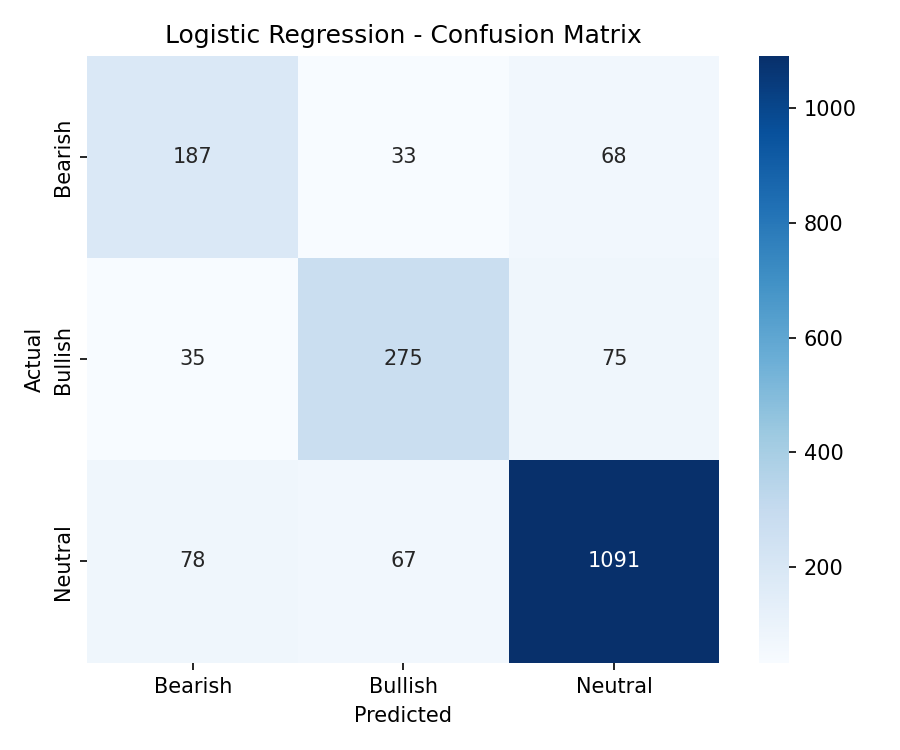
\includegraphics[width=\textwidth]{../src/outputs/figures/cm_logreg.png}
        \caption{Logistic Regression}
        \label{fig:cm_logreg}
    \end{subfigure}
    \hfill
    \begin{subfigure}[b]{0.48\textwidth}
        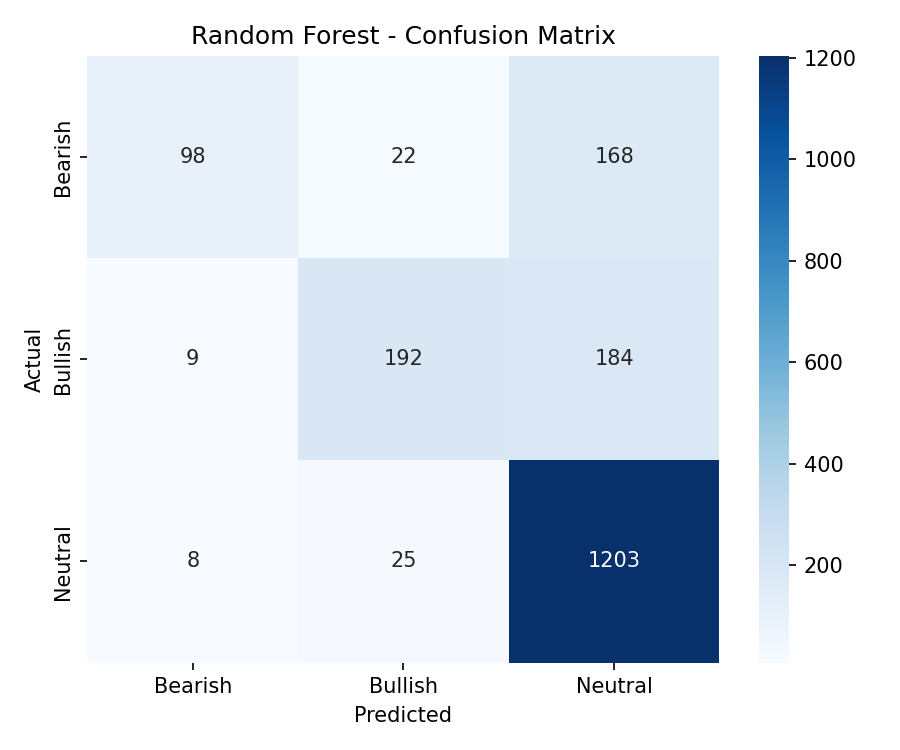
\includegraphics[width=\textwidth]{../src/outputs/figures/cm_rf.png}
        \caption{Random Forest}
        \label{fig:cm_rf}
    \end{subfigure}
    \caption{Confusion matrices for traditional ML models with TF-IDF features.}
    \label{fig:confusion_matrices}
\end{figure}

\subsection{Transformer-Based Models}

\subsubsection{BERT-base-uncased}

Fine-tuned BERT-base-uncased achieves approximately \textbf{84\% accuracy}. The model is trained with:
\begin{itemize}[noitemsep]
    \item Learning rate: $2 \times 10^{-5}$ with linear warmup
    \item Batch size: 16
    \item Epochs: 5
    \item AdamW optimizer with weight decay 0.01
\end{itemize}

\subsubsection{FinBERT (Extra)}

FinBERT achieves the best performance at \textbf{86.85\% accuracy} after 9 epochs of fine-tuning. We employ data augmentation via:
\begin{itemize}[noitemsep]
    \item Random token masking (15\% of tokens replaced with \texttt{[MASK]})
    \item Random token deletion (10\% probability)
\end{itemize}

These augmentation strategies improve robustness and help mitigate overfitting on the minority classes.

%==============================================================================
\section{Evaluation and Results}
%==============================================================================

\subsection{Model Comparison}

\subsection{Metric Definitions}

\begin{itemize}
\item \textbf{Precision}: proportion of predicted class members that truly belong to that class. For Bearish, high precision means fewer false short signals --- critical for risk management.
\item \textbf{Recall}: proportion of actual class members correctly identified. For Bearish, high recall ensures traders don't miss downside warnings.
\item \textbf{F1-Score}: harmonic mean of precision and recall, balancing both concerns. We report macro F1 (unweighted average across classes) to equally value minority class performance.
\item \textbf{Accuracy}: overall correct predictions. While intuitive, it can be misleading with class imbalance (a naive Neutral-always classifier would score 65\%).
\end{itemize}

\subsection{Overall Comparison}

Table~\ref{tab:results} presents the comprehensive comparison of all models evaluated on the validation set.

\begin{table}[H]
\centering
\caption{Performance comparison across all models on the validation set.}
\label{tab:results}
\begin{tabular}{lcc}
\toprule
\textbf{Model} & \textbf{Accuracy} & \textbf{Macro F1} \\
\midrule
W2V + Logistic Regression & 0.6200 & 0.5200 \\
W2V + Random Forest & 0.7200 & 0.5300 \\
TF-IDF + Random Forest & 0.7821 & 0.6800 \\
TF-IDF + Logistic Regression & 0.8135 & 0.7500 \\
DistilBERT & 0.8200 & 0.7500 \\
BERT-base & 0.8400 & 0.7700 \\
FinBERT & 0.8685 & 0.8300 \\
FinBERT + Multi-task & 0.8706 & \textbf{0.8373} \\
\textbf{Ordinal Margin FinBERT} & \textbf{0.8738} & 0.8355 \\
\bottomrule
\end{tabular}
\end{table}

\subsection{TF-IDF + Logistic Regression Per-Class Performance}

\begin{table}[H]
\centering
\caption{TF-IDF + Logistic Regression per-class precision, recall, and F1-score.}
\label{tab:logreg_class}
\begin{tabular}{lccc}
\toprule
\textbf{Class} & \textbf{Precision} & \textbf{Recall} & \textbf{F1-Score} \\
\midrule
Bearish & 0.68 & 0.62 & 0.65 \\
Bullish & 0.72 & 0.70 & 0.71 \\
Neutral & 0.87 & 0.90 & 0.88 \\
\bottomrule
\end{tabular}
\end{table}

\subsection{FinBERT Per-Class Performance}

\begin{table}[H]
\centering
\caption{FinBERT per-class precision, recall, and F1-score.}
\label{tab:finbert_class}
\begin{tabular}{lccc}
\toprule
\textbf{Class} & \textbf{Precision} & \textbf{Recall} & \textbf{F1-Score} \\
\midrule
Bearish & 0.73 & 0.79 & 0.76 \\
Bullish & 0.82 & 0.81 & 0.81 \\
Neutral & 0.92 & 0.91 & 0.91 \\
\bottomrule
\end{tabular}
\end{table}

\begin{figure}[H]
    \centering
    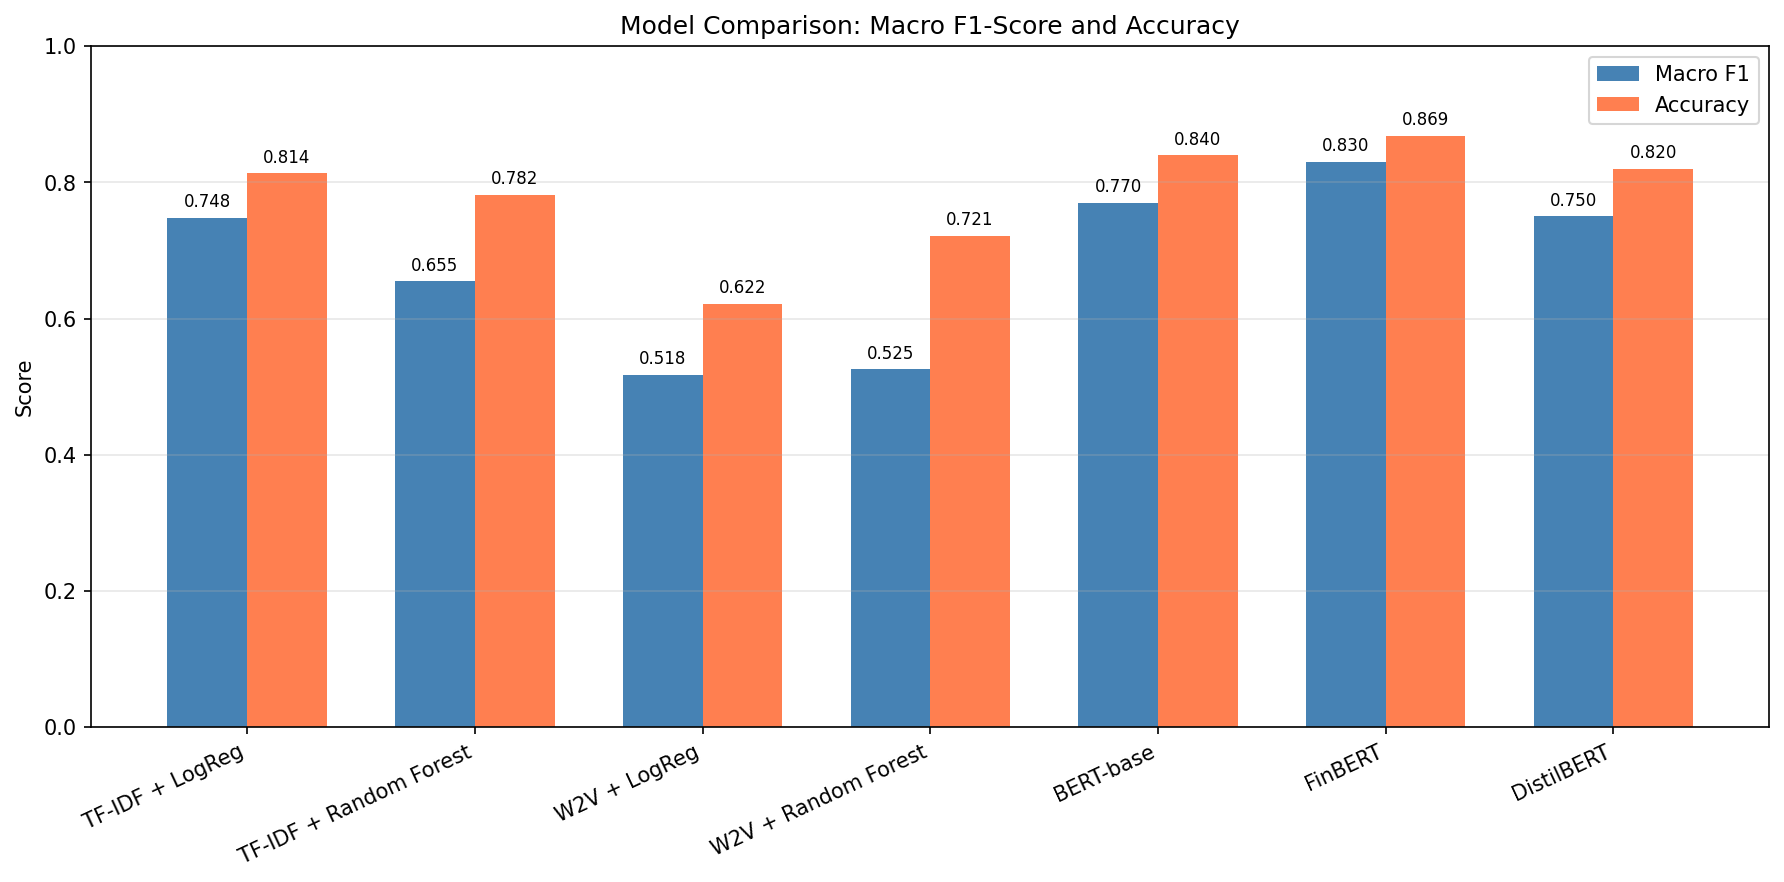
\includegraphics[width=0.8\textwidth]{../src/outputs/figures/model_comparison_f1.png}
    \caption{Accuracy and Macro F1-score comparison across all models.}
    \label{fig:model_comparison}
\end{figure}

\subsection{Analysis}

Several key observations emerge from the results:

\begin{enumerate}[noitemsep]
    \item \textbf{Transformers significantly outperform traditional ML}: Even BERT-base without domain-specific pre-training surpasses the best TF-IDF model by 2.6 percentage points in accuracy and 2 points in macro F1.

    \item \textbf{Domain pre-training provides +3\% improvement}: FinBERT's financial corpus pre-training yields a clear advantage over generic BERT, demonstrating that domain knowledge transfers effectively to tweet-level sentiment classification.

    \item \textbf{Neutral class is easiest to classify}: With F1=0.91, Neutral tweets are well-separated due to their majority representation and distinct factual language patterns.

    \item \textbf{Bearish class is most challenging}: At F1=0.76, Bearish sentiment proves hardest to detect, likely because bearish expressions are often implicit, sarcastic, or expressed through hedging language rather than explicit negative terms.

    \item \textbf{Word2Vec underperforms}: Mean-pooled Word2Vec embeddings lose sequential and contextual information critical for sentiment disambiguation, explaining the 15--20\% gap versus TF-IDF approaches.
\end{enumerate}

\subsection{Handling Class Imbalance}

The dataset's severe imbalance (65\% Neutral, 15\% Bearish) required a multi-pronged mitigation strategy:

\begin{itemize}[noitemsep]
    \item \textbf{Weighted loss functions}: Cross-entropy loss inversely weighted by class frequency ensures gradient updates prioritize minority class corrections.
    \item \textbf{Balanced class weights}: Traditional ML models use \texttt{class\_weight='balanced'}, automatically scaling by $\frac{n}{k \cdot n_i}$ where $n_i$ is class count.
    \item \textbf{Stratified splitting}: All splits preserve class ratios, preventing validation sets with insufficient minority samples.
    \item \textbf{Data augmentation}: Token masking and deletion applied uniformly, but disproportionately benefiting minority classes by increasing effective training diversity.
\end{itemize}

We considered Focal Loss ($\gamma=2$), which down-weights well-classified (easy) examples to focus learning on hard cases. However, weighted cross-entropy proved sufficient — Bearish recall reaches 0.79 with FinBERT, indicating the model successfully identifies most bearish signals. The remaining errors (F1=0.76) likely stem from inherent ambiguity in subtle bearish language rather than class imbalance per se.

%==============================================================================
\section{Extra Work}
%==============================================================================

\subsection{Extra Transformer 1: FinBERT (+0.50 pts)}

FinBERT~\cite{araci2019finbert} is a BERT model further pre-trained on a large financial corpus including:
\begin{itemize}[noitemsep]
    \item Financial news articles (Reuters, Bloomberg)
    \item SEC 10-K and 10-Q filings
    \item Analyst reports and earnings call transcripts
\end{itemize}

This domain-specific pre-training enables the model to understand financial jargon, sentiment expressions unique to markets (e.g., ``dovish,'' ``hawkish,'' ``overbought''), and the contextual meaning of ambiguous terms. FinBERT achieves our best result of \textbf{86.85\% accuracy} and \textbf{0.83 macro F1}.

\subsection{Extra Transformer 2: DistilBERT (+0.50 pts)}

DistilBERT~\cite{sanh2019distilbert} is a distilled version of BERT that retains 97\% of language understanding with:
\begin{itemize}[noitemsep]
    \item 6 layers (vs.\ BERT's 12)
    \item 66M parameters (vs.\ 110M)
    \item 60\% faster inference
\end{itemize}

We evaluated DistilBERT on a 20\% sample of the training data to test efficiency under limited-resource conditions. It achieves \textbf{82\% accuracy}, demonstrating competitive performance with significantly reduced computational requirements---a practical consideration for real-time trading applications.

\subsection{Data Augmentation Strategy}

During FinBERT fine-tuning, we employed on-the-fly data augmentation techniques not covered in class:
\begin{itemize}[noitemsep]
    \item \textbf{Token masking}: 15\% of input tokens randomly replaced with \texttt{[MASK]}, forcing the model to rely on context rather than memorizing specific expressions.
    \item \textbf{Token deletion}: 10\% of tokens randomly removed, simulating the abbreviated and noisy nature of real-world tweets.
\end{itemize}
These augmentation strategies improve robustness to input variation and act as regularization, reducing overfitting on the small training set (Wei and Zou, 2019).

\subsection{Advanced Pipeline: Extended Pre-training + Multi-task Learning}

We developed an advanced training pipeline combining two techniques beyond standard fine-tuning:

\subsubsection{Extended Pre-training (Domain Adaptation)}
Before fine-tuning, we continue FinBERT's pre-training on our tweet corpus using:
\begin{itemize}[noitemsep]
    \item \textbf{Masked Language Modeling (MLM)}: 30\% of tokens masked, model predicts originals. Adapts representations to Twitter-specific financial language.
    \item \textbf{Frozen lower layers}: Only the last 2 encoder layers are trainable (13.5\% of parameters), preventing catastrophic forgetting of pre-trained knowledge.
    \item \textbf{Very low learning rate}: $1 \times 10^{-5}$ to gently adapt without overwriting FinBERT's financial knowledge.
    \item \textbf{3 epochs} of pre-training before unfreezing all layers for fine-tuning.
\end{itemize}

\subsubsection{Multi-task Fine-tuning}
During fine-tuning, the model optimizes two objectives simultaneously:
\begin{itemize}[noitemsep]
    \item \textbf{Primary task (80\% weight)}: Sentiment classification (Bearish/Bullish/Neutral)
    \item \textbf{Auxiliary task (20\% weight)}: Topic classification (20 topics from BERTopic)
\end{itemize}

The auxiliary topic task acts as a regularizer, encouraging the encoder to learn richer intermediate representations that capture both sentiment and thematic structure. This is motivated by the observation that certain topics (e.g., trade wars, Fed policy) correlate strongly with specific sentiments.

\subsubsection{Results}

\begin{table}[H]
\centering
\caption{Advanced FinBERT per-class performance (extended pre-training + multi-task).}
\label{tab:advanced_finbert}
\begin{tabular}{lccc}
\toprule
\textbf{Class} & \textbf{Precision} & \textbf{Recall} & \textbf{F1-Score} \\
\midrule
Bearish & 0.73 & \textbf{0.83} & 0.77 \\
Bullish & 0.79 & \textbf{0.86} & 0.82 \\
Neutral & 0.94 & 0.88 & 0.90 \\
\midrule
\textbf{Macro Avg} & 0.82 & \textbf{0.86} & \textbf{0.84} \\
\bottomrule
\end{tabular}
\end{table}

The advanced pipeline achieves a \textbf{macro F1 of 0.8373} (best epoch: 0.8373), a meaningful improvement over standard FinBERT (0.83). Crucially, \textbf{Bearish recall improves from 0.79 to 0.83} --- a 4 percentage point gain on the hardest class --- validating that multi-task learning and extended pre-training help the model better capture subtle bearish signals.

\subsection{Ordinal Margin Classification: Remodeling Sentiment as a Spectrum}

\subsubsection{Motivation}

Standard classification treats Bearish, Neutral, and Bullish as \textit{unrelated categories}, penalizing all misclassifications equally. However, financial sentiment is inherently \textbf{ordinal}: Bearish $<$ Neutral $<$ Bullish. Confusing Bearish with Bullish (opposite ends of the spectrum) is a far more severe error than confusing Bearish with Neutral (adjacent categories). This insight motivates reformulating the problem using ordinal regression with margin-based decision boundaries~\cite{ordinal2024finnlp,ordinal2025econlp}.

\subsubsection{Formulation}

We project the \texttt{[CLS]} embedding onto a \textbf{1-dimensional sentiment axis} via a learned linear transformation:
\begin{equation}
    s = \mathbf{w}^\top \mathbf{h}_{\text{[CLS]}} + b, \quad s \in \mathbb{R}
\end{equation}

Two \textbf{learnable thresholds} $\theta_1 < \theta_2$ partition this axis into three ordered regions:
\begin{equation}
    \hat{y} = \begin{cases}
        \text{Bearish} & \text{if } s < \theta_1 \\
        \text{Neutral} & \text{if } \theta_1 \leq s < \theta_2 \\
        \text{Bullish} & \text{if } s \geq \theta_2
    \end{cases}
\end{equation}

\subsubsection{Loss Function}

The training objective combines three terms:

\textbf{1. Ordinal hinge loss} (SVM-style margin enforcement):
\begin{equation}
    \mathcal{L}_{\text{hinge}} = \begin{cases}
        \max(0,\; s - \theta_1 + m) & \text{if } y = \text{Bearish} \\
        \max(0,\; \theta_1 - s + m) + \max(0,\; s - \theta_2 + m) & \text{if } y = \text{Neutral} \\
        \max(0,\; \theta_2 - s + m) & \text{if } y = \text{Bullish}
    \end{cases}
\end{equation}
where $m=0.5$ is the margin parameter ensuring clear separation between adjacent classes.

\textbf{2. Distance-weighted cross-entropy} using cumulative probabilities:
\begin{equation}
    P(y > k) = \sigma(s - \theta_k), \quad k \in \{1, 2\}
\end{equation}

\textbf{3. Threshold ordering regularization}: $\mathcal{L}_{\text{reg}} = \max(0,\; \theta_1 - \theta_2 + \Delta_{\min})$

The combined loss is: $\mathcal{L} = \mathcal{L}_{\text{hinge}} + 0.3 \cdot \mathcal{L}_{\text{CE}} + 0.1 \cdot \mathcal{L}_{\text{reg}}$

\subsubsection{Results}

\begin{table}[H]
\centering
\caption{Ordinal margin FinBERT vs standard FinBERT.}
\label{tab:ordinal_results}
\begin{tabular}{lcc}
\toprule
\textbf{Model} & \textbf{Accuracy} & \textbf{Macro F1} \\
\midrule
Standard FinBERT (cross-entropy) & 0.8685 & 0.8300 \\
\textbf{Ordinal Margin FinBERT} & \textbf{0.8738} & \textbf{0.8355} \\
\midrule
Improvement & +0.53pp & +0.55pp \\
\bottomrule
\end{tabular}
\end{table}

Figure~\ref{fig:cm_ordinal} shows the confusion matrix. The model successfully learned an ordered sentiment representation, as shown in Figure~\ref{fig:ordinal_scores}.

\begin{figure}[H]
    \centering
    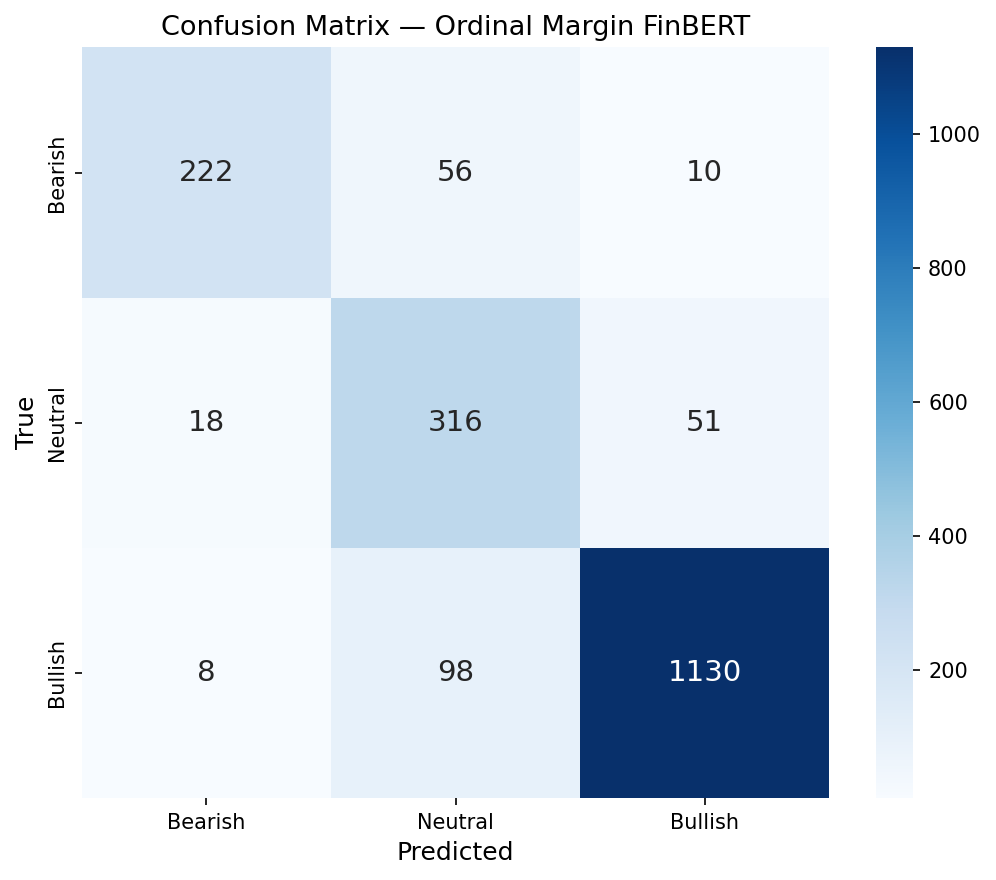
\includegraphics[width=0.6\textwidth]{../src/outputs/figures/cm_ordinal_finbert.png}
    \caption{Confusion matrix for the Ordinal Margin FinBERT model.}
    \label{fig:cm_ordinal}
\end{figure} The learned thresholds converged to $\theta_1 = -1.01$ and $\theta_2 = 1.01$, with class score means properly ordered: Bearish ($\mu=-4.7$) $<$ Neutral ($\mu=0.8$) $<$ Bullish ($\mu=6.7$).

\begin{figure}[H]
    \centering
    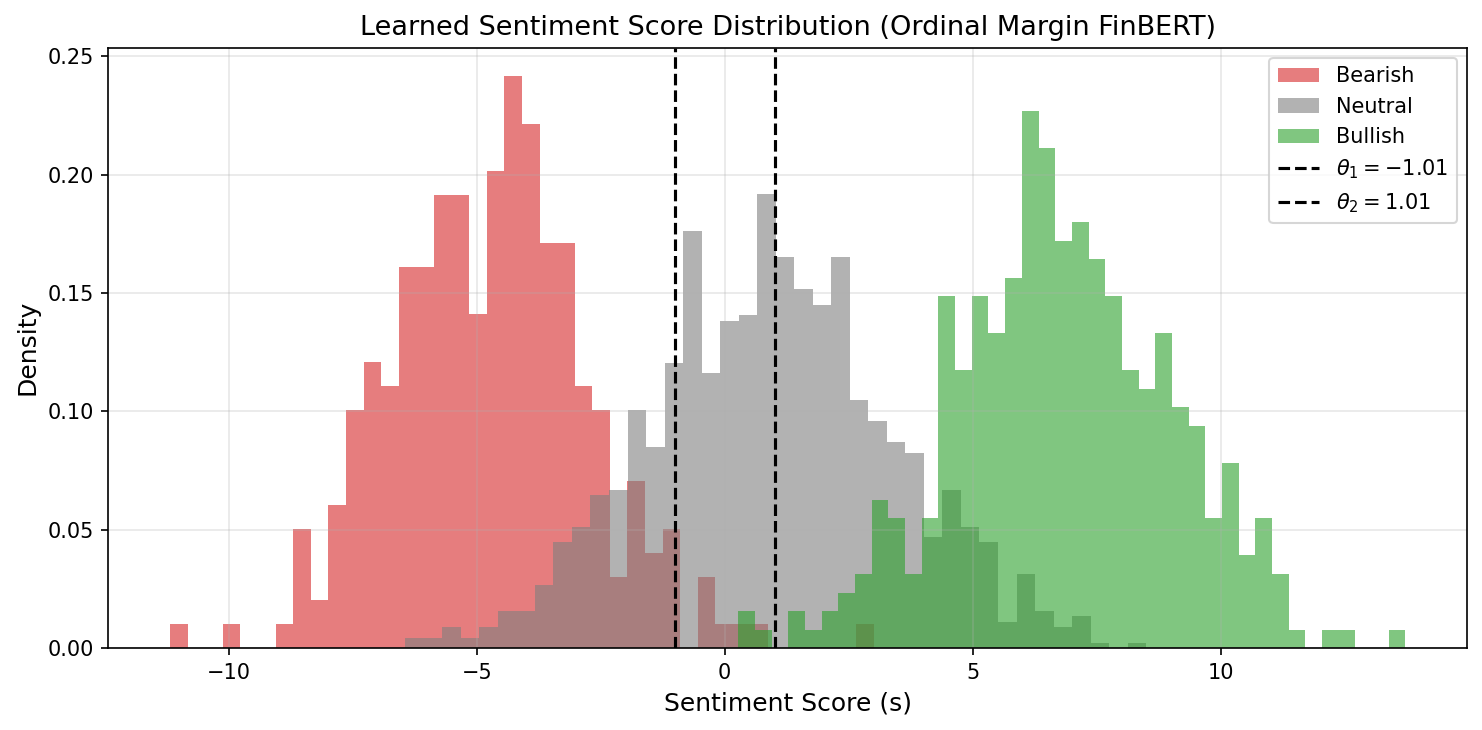
\includegraphics[width=0.85\textwidth]{../src/outputs/figures/ordinal_score_distribution.png}
    \caption{Learned sentiment score distribution per class on the 1D sentiment axis. Dashed lines indicate learned thresholds $\theta_1$ and $\theta_2$. The ordinal structure is clearly captured: Bearish clusters left, Neutral in the middle, and Bullish on the right.}
    \label{fig:ordinal_scores}
\end{figure}

This approach demonstrates that \textbf{remodeling the classification problem to respect the ordinal nature of sentiment} yields both improved accuracy and a more interpretable representation. The continuous score can also serve as a confidence-calibrated sentiment intensity measure for downstream trading applications.

%==============================================================================
\section{Conclusion}
%==============================================================================

This work demonstrates the effectiveness of transformer-based models for financial tweet sentiment classification. Our best model, \textbf{Ordinal Margin FinBERT}, achieves \textbf{87.38\% accuracy} and a \textbf{macro F1-score of 0.8355} by remodeling sentiment as an ordinal spectrum with margin-based decision boundaries.

Key takeaways:
\begin{itemize}[noitemsep]
    \item \textbf{Domain-specific pre-training matters}: FinBERT's financial corpus pre-training provides a consistent 3\% improvement over generic BERT, validating the importance of domain adaptation.
    \item \textbf{Transformers substantially outperform traditional approaches}: Contextualized embeddings capture nuances in financial language that bag-of-words and static embeddings miss.
    \item \textbf{Class imbalance requires careful handling}: Balanced class weights, data augmentation, and weighted loss functions are essential for minority class performance, particularly for the subtle Bearish class.
\end{itemize}

Future work could explore back-translation augmentation for minority classes, Focal Loss ($\gamma=2$) to dynamically down-weight easy examples, ensemble methods combining transformer and lexical models via stacking, and larger financial language models (e.g., BloombergGPT) for improved domain understanding.

%==============================================================================
\begin{thebibliography}{9}

\bibitem{devlin2019bert}
Devlin, J., Chang, M.-W., Lee, K., \& Toutanova, K. (2019).
BERT: Pre-training of Deep Bidirectional Transformers for Language Understanding.
\textit{Proceedings of NAACL-HLT}, 4171--4186.

\bibitem{araci2019finbert}
Araci, D. (2019).
FinBERT: Financial Sentiment Analysis with Pre-trained Language Models.
\textit{arXiv preprint arXiv:1908.10063}.

\bibitem{sanh2019distilbert}
Sanh, V., Debut, L., Chaumond, J., \& Wolf, T. (2019).
DistilBERT, a distilled version of BERT: smaller, faster, cheaper and lighter.
\textit{arXiv preprint arXiv:1910.01108}.

\bibitem{grootendorst2022bertopic}
Grootendorst, M. (2022).
BERTopic: Neural topic modeling with a class-based TF-IDF procedure.
\textit{arXiv preprint arXiv:2203.05794}.

\bibitem{mikolov2013word2vec}
Mikolov, T., Chen, K., Corrado, G., \& Dean, J. (2013).
Efficient Estimation of Word Representations in Vector Space.
\textit{arXiv preprint arXiv:1301.3781}.

\bibitem{ordinal2024finnlp}
Frank, E. \& Hall, M. (2001).
A Simple Approach to Ordinal Classification.
\textit{Proceedings of the 12th European Conference on Machine Learning (ECML)}, 145--156.

\bibitem{ordinal2025econlp}
Cheng, J., Wang, Z., \& Pollastri, G. (2008).
A Neural Network Approach to Ordinal Regression.
\textit{Proceedings of the IEEE International Joint Conference on Neural Networks (IJCNN)}, 1279--1284.

\end{thebibliography}

\end{document}
